\documentclass[letterpaper]{article}
\usepackage{natbib,alifexi}
\usepackage[inline]{enumitem}
\usepackage[utf8]{inputenc}
\usepackage[T1]{fontenc}
\usepackage{amsmath}
\usepackage{cases}
\usepackage{amsfonts}

\title{Pitch Scaling of Music Signals}
\author{Théo Verhelst \\
Université Libre de Bruxelles}


\begin{document}
\maketitle

\begin{abstract}
Pitch scaling is the task of modifying the frequency of a signal while keeping
its playback speed intact. Pitch scaling is an important feature of many digital
music tools, and needs to be done in real-time with the highest available
quality. In this report, we describe succinctly state-of-the-art techniques of
pitch scaling, and we explain in detail one that is particularly suited to music
signals. We also describe a Clojure implementation of this technique. This
technique uses phase vocoder for time-scaling and 3rd order spline interpolation
for resampling.
\end{abstract}

\section{Introduction}
Pitch scaling is a process that changes the frequency of a signal without
modifying its speed. The main difficulty of pitch scaling is to make the
synthesised signal as natural as the original, so that it sounds like as if it
was recorded or created on this new pitch. More precisely, the timbre and the
speed of the signal need to be preserved.
\paragraph{}
One application of pitch scaling is to scale the pitch of an instrument
recording in a music production software, in order to tune it to the other
instruments, or for any other musical purpose. But the main use of pitch scaling
is probably in DJ software: one can change the pitch of a track, and therefore
its key, in order to make the transition to the next track easier and smoother.
\paragraph{}
The most straightforward way to change the pitch of an audio signal is to
resample the signal and playing it back at its original rate \citep{DM}. But
both pitch and speed are modified at the same time. Thus, we need a more
sophisticated technique in order to preserve the playback speed constant.
\paragraph{}
In contrast to pitch scaling, time-scale modification (TSM) is a process that
modifies the speed of a signal without modifying its pitch and its timbre.
TSM has been subject to many more studies than pitch scaling, but we base our
work on these studies, since it is possible to show that both processes are
mathematically equivalent. Indeed, in order to change the pitch of a signal, one
can use a well-known TSM method, and then resample the signal.

\section{Time-scale modification techniques}
TSM techniques can be grouped in two main categories: \emph{time-domain TSM} and
\emph{frequency-domain TSM}.
\paragraph{}
Time-domain TSM extracts portions of the input signal at a frequency defined by
the scaling factor, and places them in the output signal. This technique is
particularly suited to monophonic, harmonic signal, as it preserves almost
perfectly the timbre of the signal. The basic time-domain algorithm,
\emph{overlap-and-add} (or \emph{OLA}), suffers from phase jumps artifacts, but there are many
variations of this algorithm that avoid this effect. But all of them are only
able to correct phase jumps on the most prominent frequency, i.e. the fundamental
frequency of the signal. Phase jumps can still occur in less important frequencies,
i.e. the harmonics, which is clearly audible. OLA-base algorithms are thus not
suited to polyphonic signals, since they contains more harmonics than monophonic
ones. Furthermore, non-harmonic signals, such as drums or percussive instruments, have non-periodic patterns. These patterns
are known as \emph{transients}. A typical time-domain TSM technique leads to
transient doubling or skipping (depending on the scaling factor), since these
techniques periodically repeat or discard some small parts of the signal. This
can be avoided by taking a very short frame size.
\paragraph{}
Frequency-domain TSM is based on the short-time Fourier transform (STFT). It
splits the signal in small chunks, and computes the Fourier transform of each
of these chunks, in order to get a discrete frequency-domain representation of the
signal. Often, the technique also uses the \emph{phase vocoder} in order to
refine the frequencies estimates, and are thus named \emph{phase-vocoder
time-scale modification}, or \emph{PV-TSM}, or simply phase vocoder. The idea is
to preserve phase continuity across all frequencies, and not only on the most
prominent frequency as in time-domain TSM, by exploiting the frequency-domain
representation of the sound. PV-TSM behaves well on polyphonic signals, but are
subject to vertical phase incoherence, i.e. the relationship between the phases
of different frequencies at a point of time is not preserved, leading to audible
artifacts, known as \emph{phasiness}, or \emph{loss of presence}.

\section{General procedure}
Pitch scaling process is split in two steps: \begin{enumerate*}[label=\arabic*)]
\item apply a TSM procedure \item resample the signal\end{enumerate*}. Let
\(\alpha\) be the scaling factor. We first apply a TSM procedure with parameter
\(\alpha\), so that the playback speed is modified, while the pitch is left
unmodified. Then, we resample the signal by a factor \(1/\alpha\), so that the
playback speed of the signal is the same as the original, but the pitch is
multiplied by \(\alpha\).
\paragraph{}
For the TSM part, we use a simple phase vocoder with phase propagation. For the
resampling part, we use an interpolator based on 3rd order splines. These are
explained below.

\section{Time-scale modification}
\subsection{Basics of time-scale modification}
\paragraph{Notation:} Let
\[[a:b]:=\{a,a+1,\dots,b-1,b\}\quad\forall a,b\in\mathbb{Z}:a<b\]
and
\[[a:b[\;:=\{a,a+1,\dots,b-1\}\quad\forall a,b\in\mathbb{Z}:a<b\]
\paragraph{}
First, we have to define the basic concepts involved in time-scaling. Let the
function \(x:\mathbb{Z}\to[-1, 1]\) be signal to time-scale. In practice,
the analysed audio signal has a finite duration of \(L\in\mathbb{N}\) samples.
Thus we define \(x(n)=0\,\forall n\in\mathbb{Z}\setminus [0:L[ \) for the sake
of simplicity. We want to construct the output signal
\(y:\mathbb{Z}\to[-1, 1]\) that have the same frequency-domain properties as
\(x\), but being stretched in time by the factor \(\alpha\).
\paragraph{}
Almost all TSM techniques are based on the following procedure: first, \(x\)
is divided in \emph{analysis frames} \(x_m,\,m\in\mathbb{Z}\) having each a
length of \(N\) samples, and these analysis frames are spaced by an
\emph{analysis hop size} \(H_a\):
\begin{equation}x_m(n)=\begin{cases}
		x(mH_a + n) & \text{if }n\in [0:N[ \\
		0           & \text{otherwise}
\end{cases}\end{equation}
Then, we could want to put these frames in the output signal by spacing them by
the synthesis hop size \(H_s\), achieving the correct time-scale modification. But this
would cause very audible phase discontinuities, since the end of a frame would
no longer match with the beginning of the next frame. Thus, we need to modify
the analysis frames \(x_m\) into \emph{synthesis frames} \(y_m\) before adding
them to the output signal \(y(n)\):
\begin{equation}
		y(n) = \sum_{m\in\mathbb{Z}}y_m(n-mH_s)
\end{equation}
\begin{figure}[h]
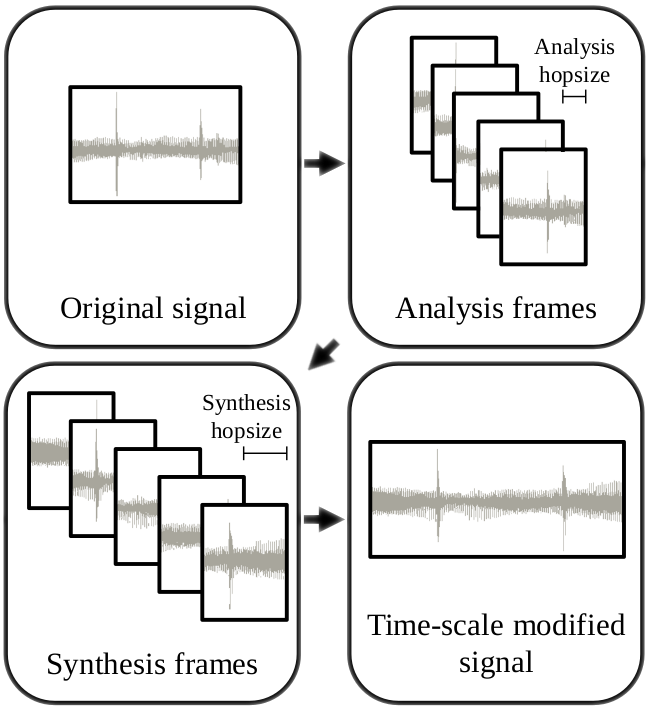
\includegraphics[width=\linewidth]{pipeline.png}
\caption{General procedure of time-scale modification.}
\end{figure}
\paragraph{}
\(H_s\) is usually set to \(N/2\) or \(N/4\), in order to have a constant
overlap between the synthesis frames. And since we know that
\(\alpha=\frac{H_s}{H_a}\), we then have \(H_a=\frac{H_s}{\alpha}\).
\paragraph{}
The method used to transform \(x_m\) into \(y_m\) is critical, as it determines
the quality of the result. In addition to phase discontinuities, it must also
compensate gain fluctuations: if no care is taken, two overlapping frames may
have a higher gain in the overlapping part than in the rest of the signal.
A common procedure to compensate gain fluctuations is to multiply each modified
frame by a windowing function \(w:\mathbb{N}\to[0,1]\) before adding them to the
output signal \(y\):
\begin{equation}
		\label{synthesis}
		y(n) = \sum_{m\in\mathbb{Z}}w(n-mH_s)y_m(n-mH_s)
\end{equation}
 The Hann window is widely used for this purpose, and is defined as
\begin{equation}
\label{hann}
w(n)=\begin{cases}
	  0.5(1-cos(\frac{2\pi n}{N-1}))\text{ if }n\in[0:N[\\
	  0 \text{ otherwise}\end{cases}
\end{equation}
The Hann window has the property that if we add Hann windows spaced by \(N/2\)
in their domain, the sum of the overlapping parts we be equal to one:
\begin{equation}
		\forall n\in\mathbb{Z}\quad\sum_{i\in\mathbb{Z}}w(n + i\frac{N}{2}) = 1
\end{equation}
This property is essential to the equation \eqref{synthesis}: if not satisfied,
the output signal may be multiplied by more than one in some places.
\begin{figure}[h]
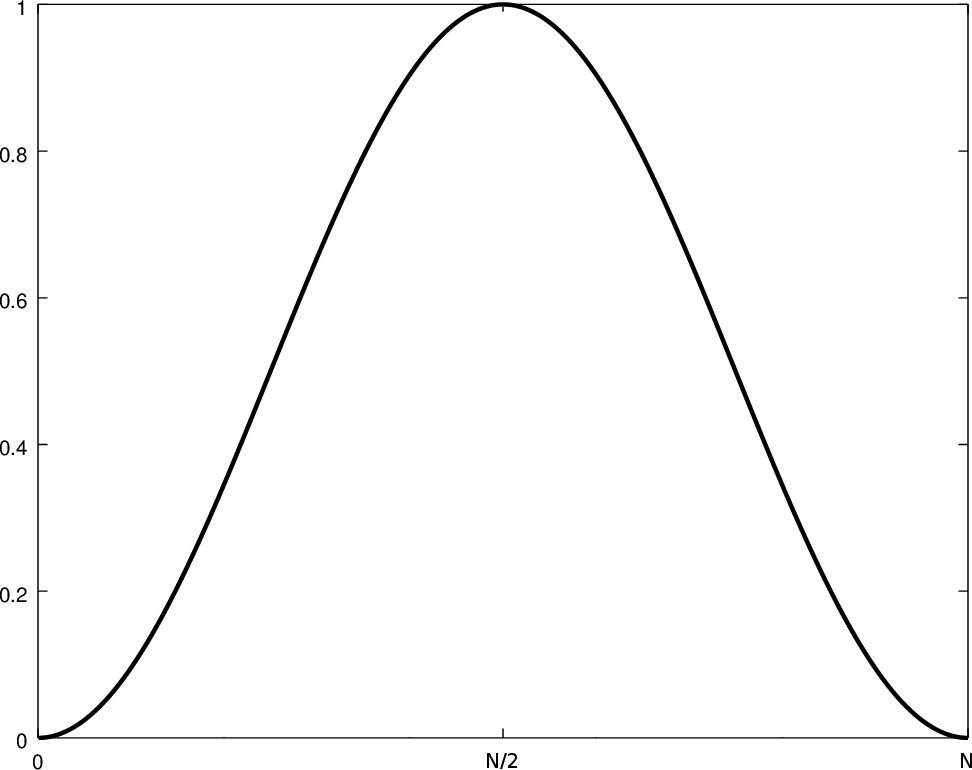
\includegraphics[width=\linewidth]{hann.png}
\caption{The Hann window function.}
\end{figure}

\subsection{Phase-vocoder time-scale modification}
The phase vocoder is a common frequency-domain technique used to derive the
\emph{synthesis frames} \(y_m\)  from the analysis frames \(x_m\). The idea
is to compute the spectrum of the frame with the Fourier transform, and change
the phases of this spectrum so that the signal re-synthesised from this modified
spectrum has no phase jump with the following and previous frames.
\paragraph{Short-time Fourier transform}
The spectrum of a signal is the frequency-domain representation of
a time-domain signal, and is composed by the amplitudes and phases of the
Fourier series decomposition of the signal. The Fourier transform of
discrete-time signals is primarily defined for signals of length \(N\):
\begin{equation}
	  X(k) = \sum_{n=0}^{N-1}x(n)\exp(-2\pi ikn/N)
\end{equation}
where \(k\in [0:N[\) denotes the frequency index (see \eqref{frequency_index}). This yields \(k\) complex
numbers, where \(|X(k)|\) is the magnitude of the \(k\)th frequency, and
\(\arg(X(k))\in[0,1[\) is the phase of the \(k\)th frequency. Note that we use
phases in the unit range because we also manipulate frequencies in Hertz, and
we don't want to divide the phase by \(2\pi\) each time we use it in an equation
involving a frequency. Thus, we have
\begin{equation}
		X(k)= |X(k)|\exp(2\pi \text{i} \arg(X(k)))
\end{equation}
\paragraph{}
As required by the time-scaling algorithm, we will apply the Fourier transform
on small portions of the signal. We could want to do apply directly the
transform on analysis frames \(x_m\):
\begin{equation*}
X(m,k)=\sum_{n=0}^{N-1}x_m(n)\exp(-2\pi ikn/N)
\end{equation*}
But this can lead to unexpected high amplitudes in the high frequencies:
the Fourier transform works as if the signal was periodic with a period \(N\),
i.e. as if we where computing the Fourier series of a signal
\begin{equation}
\tilde x:\mathbb{Z}\to\mathbb{R}:n\mapsto x_m(n\mod N)
\end{equation}
which can have high amplitude in high frequencies around
\(n=aN\;\forall a\in\mathbb{Z}\).
A solution is to apply a windowing function to the analysis frame, so that the
signal is always zero at the frame boundaries:
\begin{equation}
    X(m,k) = \sum_{n=0}^{N-1}x_m(n)w(n)\exp(-2\pi ikn/N)
\end{equation}
\(X(m,k)\) is the coefficient of the \emph{short-time Fourier transform} of
the signal \(x\) at time \(m\) and at frequency \(k\). It is also named a
\emph{time-frequency bin}. \(w\) is a windowing function, usually the Hann
window as defined in \eqref{hann}
\paragraph{}
Note that the frequency index \(k\) corresponds to the physical frequency
\begin{equation}
		\label{frequency_index}
    F_{\text{coef}}(k) = \frac{F_s k}{N}
\end{equation}
and the frame index \(m\) corresponds to the physical time
\begin{equation}
    T_{\text{coef}}(m) = \frac{H_a m}{F_s}
\end{equation}
\paragraph{Synthesis with modified frames}
Our goal is to compute the synthesis frequency bins \(Y(m,k)\) from the analysis
frequency bins \(X(m,k)\), so that the signal synthesised with the inverse
Fourier transform from these synthesis frequency bins has no phase incoherence
from one frame to the next. Since we are only interested in phase adjustment,
we can already set
\begin{equation}
    |Y(m,k)| = |X(m,k)|
\end{equation}
We also have to determine the phase \(\arg(Y(m,k))\), so that we can synthesise
the synthesis frame \(y_m\) from the synthesis frequency bins \(Y(m,k)\) with
the inverse Fourier transform:
\begin{equation}
		y_m(n)=\frac{1}{N}\sum_{k=0}^{N-1}Y(m,k)\exp(2\pi\text{i}kn/N)
\end{equation}
and then reconstruct the output signal with the equation \eqref{synthesis}.

\paragraph{Instantaneous frequency}
The phase adjustment involves the observation that the short-time Fourier
transform yields coefficients for a finite quantity of frequencies, and that may
be insufficient to characterise exactly the underlying sinusoids involved in the
Fourier series decomposition of the signal. However, it is possible to refine
the frequency of the \(k\)th frequency index by using the phases of the current
and next frame. This refined frequency is called the \emph{instantaneous
frequency} and is denoted by \(F_{\text{coeff}}^{\text{IF}}(m,k)\).
\paragraph{Notation:}
Let \[\phi_m:=\arg(X(m,k))\]
In order to find the instantaneous frequency, we first can observe that for
any frequency bin \(X(m,k)\), we can compute its \emph{unwrapped phase advance},
that is, the phase increment that should occur from the time
\(T_{\text{coef}}(m)\) to the time \(T_{\text{coef}}(m+1)\), according to the
frequency estimate \(F_{\text{coef}}(k)\):
\begin{equation}
    \phi^{\text{inc}}=F_{\text{coef}}(k) \Delta t
\end{equation}
where \(\Delta t\) is analysis hop time given is seconds:
\begin{equation}
    \Delta t=H_a/F_s
\end{equation}
Since we know the phase \(\phi_m\), we can compute the predicted phase at
the time \(T_{\text{coef}}(m)\):
\begin{equation}
    \phi^{\text{pred}}_m=\phi_m + \phi^{\text{inc}}
\end{equation}
But because of the lack of precision of the phase vocoder, this predicted phase
may not be equal to \(\phi_{m+1}\) when mapped in the range \([0, 1[\).
We can then compute the difference with the effective phase \(\phi_{m+1}\), and
this difference is called the \emph{phase error} (or \emph{heterodyned phase
increment}):
\begin{equation}
    \phi^{\text{err}}=\Psi(\phi_{m+1} - \phi^{\text{pred}}_m)
\end{equation}
where the function \(\Psi\) is the \emph{principal argument function} that maps
the phase difference to the range \([-0.5, 0.5]\).
Here is a possible implementation of \(\Psi\):
\begin{equation}
    \Psi:\mathbb{R}\to[-0.5,0.5]:\phi\mapsto \phi - \lceil \phi-0.5 \rceil
\end{equation}
From this phase error, we can compute the \emph{instantaneous frequency}: this
is a refinement of \(F_{\text{coef}}(k)\), in an attempt to determine the
frequency of the underlying sinusoid by taking the phase error into account.
This sinusoid should have a phase of
\(\phi_m\) at the time \(T_{\text{coef}}(m)\) and a phase \(\phi_{m+1}\) at
the time \(T_{\text{coef}}(m+1)\).
\begin{align}
    &F_{\text{coeff}}^{\text{IF}}(m,k)=\frac{\phi^{\text{inc}} + \phi^{\text{err}}_m}{\Delta t}\\
    &=F_{\text{coef}}(k) + \frac{\phi^{\text{err}}_m}{\Delta t}\\
    &=F_{\text{coef}}(k) + \frac{\Psi(\phi_{m+1} - \phi_m - \phi^{\text{inc}})}{\Delta t}
\end{align}

\paragraph{Phase adjustment}

\subsection{Result and limitations}
\subsection{Further improvements}

\section{Resampling}
The goal of resampling is to reconstruct a continuous-time signal from the given
discrete-time samples, and then sample this signal again with another sampling
rate. More formally, we want to construct the continuous-time signal
\begin{equation}\hat x:\mathbb{R}\to\mathbb{R}\end{equation}
such that
\begin{equation}x(n) = \hat x(Tn) \;\forall n\in\mathbb{Z}\end{equation}
where \(T\) is the sampling period (the inverse of the sampling rate). Then, we
sample a new signal \(y\) at a sampling period \(T'\):
\begin{equation*}y(n) = \hat x(T'n) \;\forall n\in\mathbb{Z}\end{equation*}
\paragraph{}
In order to construct the continuous-time signal, we need an interpolator. There
exists various interpolators, such as truncated sinc, linear-interpolator,
b-spline interpolator, Lagrange interpolator. We chose 3rd order spline
interpolator, for its simple implementation, although it does not give the best
results for musical signal interpolation.
\paragraph{}
For 3rd order spline interpolation, we search the factors of a 3rd-degree
polynomial for each pair of consecutive signal values \((x(n),\,x(n+1))\), such
that this polynomial passes through these values. For the sake of the notation,
let
\begin{equation*}
y_0=x(n-1);\;y_1=x(n);\;y_2=x(n+1);\;y_3=x(n+2)
\end{equation*}
We search a function
\begin{equation}
\label{interpolation_poly}
f:[0, 1]\to\mathbb{R}:t\mapsto \sum_{i=0}^{3}\alpha_i t^i
=\alpha_0+\alpha_1 t+\alpha_2t^2+\alpha_3t^3
\end{equation}
In order to determine the value of the factors \(\alpha_i\), we need to set four
constraints on the function \(f\):
\begin{numcases}{ }
f(0)=y_1\label{constr1}\\
f(1)=y_2\label{constr2}\\
f'(0)=\frac{y_2-y_0}{2}\label{constr3} \\
f'(1)=\frac{y_3-y_1}{2}\label{constr4}
\end{numcases}
\eqref{constr1} and \eqref{constr2} are natural constraints of spline
interpolator: we want that the interpolating function passes through the
supplied values
\((x(n),\,x(n+1))\). But in order to determine the factors \(\alpha_i\), we need
two more constraints. One solution is to use Hermitian splines, that is,
the derivative of \(f\) at \(t\in\{0, 1\}\) is equal to the derivative of a
straight line between the previous and the next point (\eqref{constr3} and
\eqref{constr4}). By expressing the equations as a matrix equation,
we can find that
\begin{align}
\begin{bmatrix}
	\alpha_0\\\alpha_1\\\alpha_2\\\alpha_3
\end{bmatrix}
&=
\begin{bmatrix}
	 1 &  0 &   0 &  0   \\
	 0 &  0 & 0.5 &  0   \\
	-3 &  3 &  -1 & -0.5 \\
	 2 & -2 & 0.5 &  0.5 \\
\end{bmatrix}
\begin{bmatrix}
	y_1\\y_2\\y_2-y_0\\y_3-y_1
\end{bmatrix}
\end{align}
For each pair of samples, we just have to compute the four factors \(\alpha_i\)
with this equation, and then evaluate the function \(f\) as in
\eqref{interpolation_poly}, at a value of \(t\) corresponding to the new
sampling rate.
\section{Clojure implementation}
\subsection{The Clojure programming language}
\subsection{Overtone}
\subsection{Implementation of pitch scaling}

\section{Results}
\section{Conclusion}

\footnotesize
\bibliographystyle{apalike}
\bibliography{Report}


\end{document}
